\begin{center}
\Huge
Sammenhæng mellem $f$ og $f'$.
\end{center}

\section*{Grafer}
\stepcounter{section}

I nogle tilfælde vil vi kun kende graferne for $f$ og $f'$, og ud fra dette skal vi afgøre, hvilken af graferne der er graf for $f$ og graf for $f'$. Lad os betragte et eksempel.
\begin{exa}
	Graferne for $f$ og $f'$ kan ses af Fig. \ref{fig:grafer}.
	\begin{figure}[H]
		\centering
		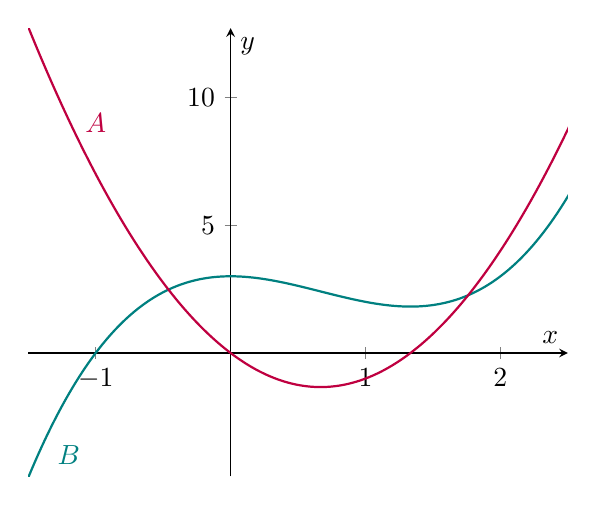
\begin{tikzpicture}
			\begin{axis}[
			axis lines = middle, 
			xlabel = {$x$},
			ylabel = {$y$},
			xmin = -1.5, xmax = 2.5]
				\addplot[color = teal, samples = 1000, thick] {x^3-2*x^2+3};
				\addplot[color = purple, samples = 1000, thick] {3*x^2-4*x};
				\node[color = purple] at (axis cs: -1,9) {$A$};
				\node[color = teal] at (axis cs: -1.2,-4) {$B$};
			\end{axis}
		\end{tikzpicture}
		\caption{Grafer for $f$ og $f'$}
		\label{fig:grafer}
	\end{figure}
	Vi skal afgøre hvilken af graferne $A$ og $B$ der tilhører $f$ og $f'$. Vi ved, at $f'(x) = 0$, når grafen for $f$ er i et ekstremumspunkt. Vi kan se, at grafen $B$ har et toppunkt i $x=0$ og et 
	minimum omkring $x=1.3$. Grafen $A$ skærer $x$-aksen i netop disse punkter. Derfor må grafen for $f$ være $B$ og grafen for $f'$ må være $A$. 
\end{exa}

Vi skal også ud fra en monotonilinje kunne skitsere en mulig graf for en funktion
\begin{exa}
	Vi får givet følgende monotonilinje og ønsker at bestemme en mulig graf for funktionen $f$. 
	\begin{center}
		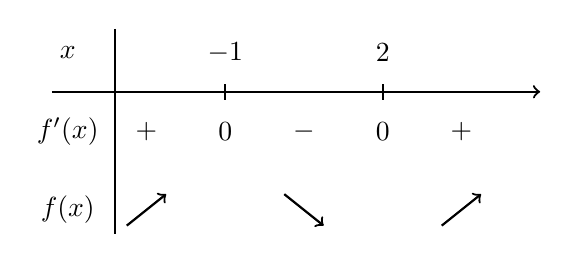
\begin{tikzpicture}
			\node at (0,0) {$x$};
			\node at (0,-1) {$f'(x)$};
			\node at (0,-2) {$f(x)$};
			\node at (2,0) {$-1$};
			\node at (4,0) {$2$};
			\node at (2,-1) {0};
			\node at (4,-1) {0};
			\node at (1,-1) {$+$};
			\node at (3,-1) {$-$};
			\node at (5,-1) {$+$};
			\draw[->,thick] (-0.2,-0.5) to (6,-0.5);
			\draw[thick] (2,-0.6) to (2,-0.4);
			\draw[thick] (4,-0.6) to (4,-0.4);
			\draw[thick] (0.6,0.3) to (0.6,-2.3);
			\draw[->,thick] (0.75,-2.2) to (1.25,-1.8);
			\draw[->,thick] (2+0.75,-1.8) to (2+1.25,-2.2);
			\draw[->,thick] (4+0.75,-2.2) to (4+1.25,-1.8);
		\end{tikzpicture}
	\end{center}
	Vi kan se, at grafen skal have ekstrema i $-1$ og $2$ samt være voksende før og efter de to ekstrema og aftagende mellem. Vi skitserer en mulig graf, som kan ses af Fig. \ref{fig:skitse}.
	\begin{figure}[H]
		\centering
		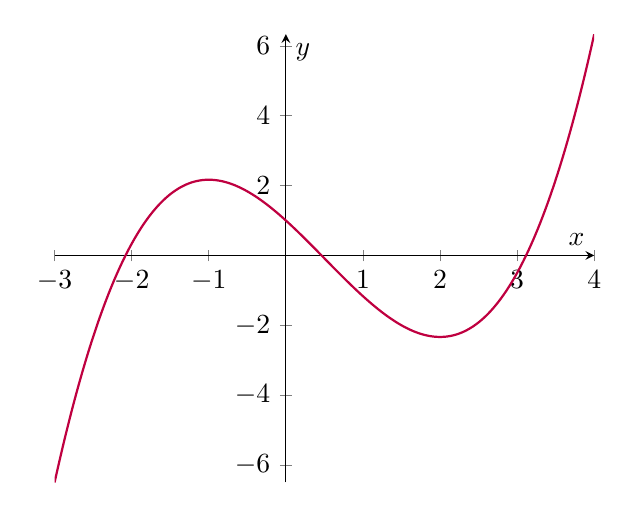
\begin{tikzpicture}
			\begin{axis}[
			axis lines = middle,
			xmin = -3, xmax = 4, 
			xlabel = {$x$},
			ylabel = {$y$}]
				\addplot[color = purple, thick, domain = -3:4, samples = 1000] {(1/3)*x^3-(1/2)*x^2-2*x+1};
			\end{axis}
		\end{tikzpicture}
		\caption{Mulig graf for funktionen med givet monotonilinje}
		\label{fig:skitse}
	\end{figure}
\end{exa}

\newpage
\section*{Opgave 1}

\begin{enumerate}[label=\roman*)]
	\item Skitsér en mulig graf for funktionen $f$ med monotonilinjen
	\begin{center}
		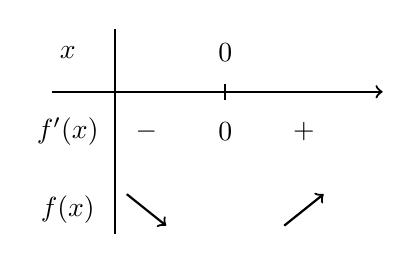
\begin{tikzpicture}
			\node at (0,0) {$x$};
			\node at (0,-1) {$f'(x)$};
			\node at (0,-2) {$f(x)$};
			\node at (2,0) {$0$};
			\node at (2,-1) {0};
			\node at (1,-1) {$-$};
			\node at (3,-1) {$+$};
			\draw[->,thick] (-0.2,-0.5) to (4,-0.5);
			\draw[thick] (2,-0.6) to (2,-0.4);
			\draw[thick] (0.6,0.3) to (0.6,-2.3);
			\draw[->,thick] (0.75, -1.8) to (1.25,-2.2);
			\draw[->,thick] (2+0.75,-2.2) to (2+1.25,-1.8);
		\end{tikzpicture}
	\end{center}
	\item Skitsér en mulig graf for funktionen $f$ med monotonilinjen
	\begin{center}
		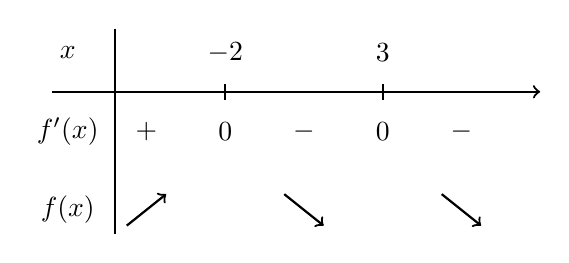
\begin{tikzpicture}
			\node at (0,0) {$x$};
			\node at (0,-1) {$f'(x)$};
			\node at (0,-2) {$f(x)$};
			\node at (2,0) {$-2$};
			\node at (4,0) {$3$};
			\node at (2,-1) {0};
			\node at (4,-1) {0};
			\node at (1,-1) {$+$};
			\node at (3,-1) {$-$};
			\node at (5,-1) {$-$};
			\draw[->,thick] (-0.2,-0.5) to (6,-0.5);
			\draw[thick] (2,-0.6) to (2,-0.4);
			\draw[thick] (4,-0.6) to (4,-0.4);
			\draw[thick] (0.6,0.3) to (0.6,-2.3);
			\draw[->,thick] (0.75,-2.2) to (1.25,-1.8);
			\draw[->,thick] (2+0.75,-1.8) to (2+1.25,-2.2);
			\draw[->,thick] (4+0.75,-1.8) to (4+1.25,-2.2);
		\end{tikzpicture}
	\end{center}
	\item Skitsér en mulig graf for funktionen $f$ med monotonilinjen
	\begin{center}
		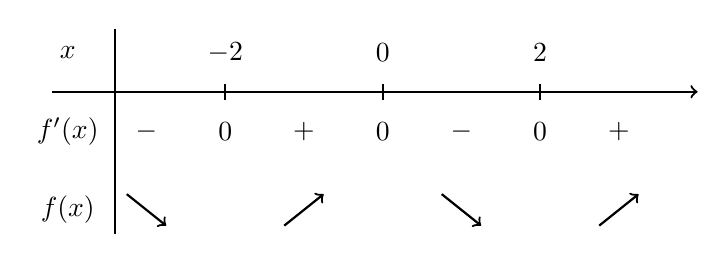
\begin{tikzpicture}
			\node at (0,0) {$x$};
			\node at (0,-1) {$f'(x)$};
			\node at (0,-2) {$f(x)$};
			\node at (2,0) {$-2$};
			\node at (4,0) {$0$};
			\node at (6,0) {$2$};
			\node at (2,-1) {0};
			\node at (4,-1) {0};
			\node at (6,-1) {0};
			\node at (1,-1) {$-$};
			\node at (3,-1) {$+$};
			\node at (5,-1) {$-$};
			\node at (7,-1) {$+$};
			\draw[->,thick] (-0.2,-0.5) to (8,-0.5);
			\draw[thick] (2,-0.6) to (2,-0.4);
			\draw[thick] (4,-0.6) to (4,-0.4);
			\draw[thick] (6,-0.6) to (6,-0.4);
			\draw[thick] (0.6,0.3) to (0.6,-2.3);
			\draw[->,thick] (0.75,-1.8) to (1.25,-2.2);
			\draw[->,thick] (2+0.75,-2.2) to (2+1.25,-1.8);
			\draw[->,thick] (4+0.75,-1.8) to (4+1.25,-2.2);
			\draw[->,thick] (6+0.75,-2.2) to (6+1.25,-1.8);
		\end{tikzpicture}
	\end{center}
	\item Skitsér en mulig graf for funktionen $f$ med monotonilinjen
	\begin{center}
		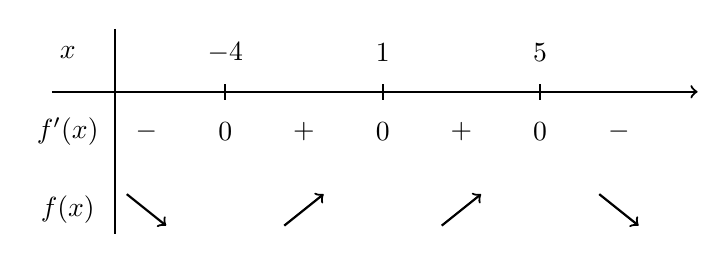
\begin{tikzpicture}
			\node at (0,0) {$x$};
			\node at (0,-1) {$f'(x)$};
			\node at (0,-2) {$f(x)$};
			\node at (2,0) {$-4$};
			\node at (4,0) {$1$};
			\node at (6,0) {$5$};
			\node at (2,-1) {0};
			\node at (4,-1) {0};
			\node at (6,-1) {0};
			\node at (1,-1) {$-$};
			\node at (3,-1) {$+$};
			\node at (5,-1) {$+$};
			\node at (7,-1) {$-$};
			\draw[->,thick] (-0.2,-0.5) to (8,-0.5);
			\draw[thick] (2,-0.6) to (2,-0.4);
			\draw[thick] (4,-0.6) to (4,-0.4);
			\draw[thick] (6,-0.6) to (6,-0.4);
			\draw[thick] (0.6,0.3) to (0.6,-2.3);
			\draw[->,thick] (0.75,-1.8) to (1.25,-2.2);
			\draw[->,thick] (2+0.75,-2.2) to (2+1.25,-1.8);
			\draw[->,thick] (4+0.75,-2.2) to (4+1.25,-1.8);
			\draw[->,thick] (6+0.75,-1.8) to (6+1.25,-2.2);
		\end{tikzpicture}
	\end{center}
\end{enumerate}

\section*{Opgave 2}

På følgende koordinatsystemer kan man se graferne for $f$ og $f'$. Afgør for hvert koordinatsystem hvilken af graferne der tilhører $f$ og hvilken af graferne der tilhører $f'$. 

\begin{center}
	\resizebox{0.45\textwidth}{!}{
		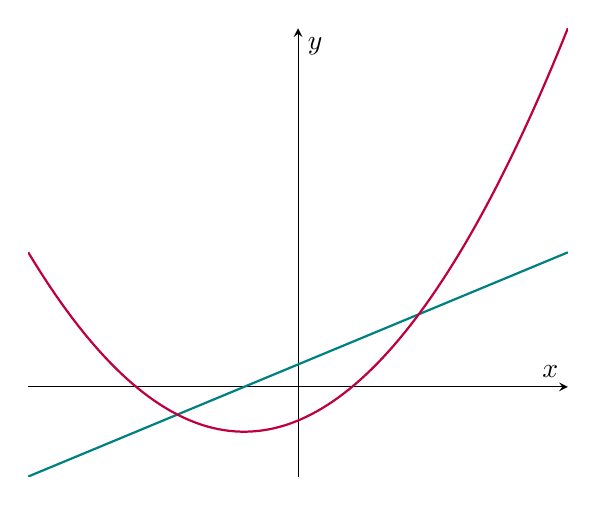
\begin{tikzpicture}
			\begin{axis}[
			axis lines = middle, 
			xlabel = {$x$},
			ylabel = {$y$},
			ticks = none]
				\addplot[color = teal, samples = 100, thick] {2*x+2};
				\addplot[color = purple, samples = 100, thick] {x^2+2*x-3};
			\end{axis}
		\end{tikzpicture}
	}
	\resizebox{0.45\textwidth}{!}{
		\begin{tikzpicture}
			\begin{axis}[
			axis lines = middle, 
			xlabel = {$x$},
			ylabel = {$y$},
			xmin = -0.5, xmax = 3,
			ticks = none]
				\addplot[color = teal, samples = 500, thick, domain = 0.01:3] {ln(x)-x^2-2};
				\addplot[color = purple, samples = 500, thick, domain  = 0.1:3] {1/x - 2*x};
			\end{axis}
		\end{tikzpicture}
	}
	\resizebox{0.45\textwidth}{!}{
		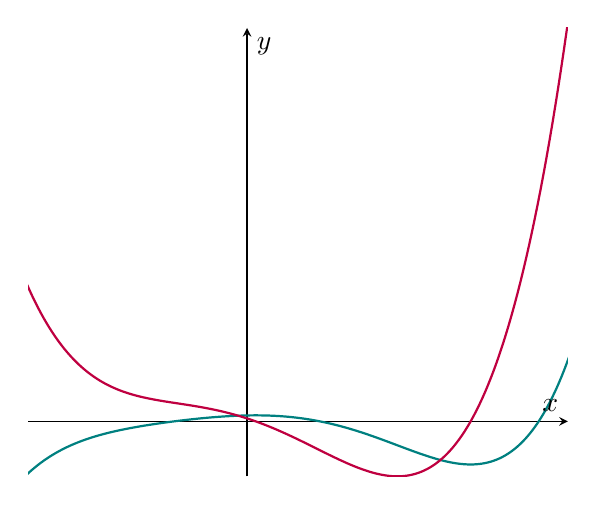
\begin{tikzpicture}
			\begin{axis}[
			axis lines = middle, 
			xlabel = {$x$},
			ylabel = {$y$},
			xmin = -1.5, xmax = 2.2,
			ticks = none
			]
				\addplot[color = teal, samples = 500, thick] {4*x^5-9*x^3-16*x^2+2*x+4};
				\addplot[color = purple, samples = 500, thick] {4*5*x^4-9*3*x^2-16*2*x+2};
			\end{axis}
		\end{tikzpicture}
	}
	\resizebox{0.45\textwidth}{!}{
		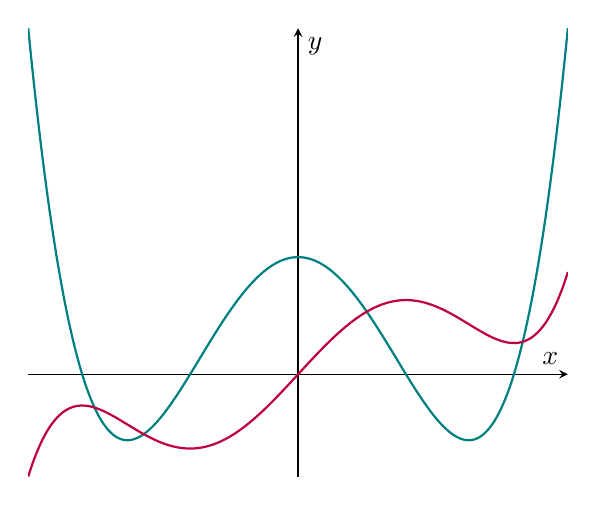
\begin{tikzpicture}
			\begin{axis}[
			axis lines = middle, 
			xlabel = {$x$},
			ylabel = {$y$},
			ticks = none,
			]
				\addplot[color = teal, samples = 500, thick, domain = -2.5:2.5] {(x-1)*(x+1)*(x-2)*(x+2)};
				\addplot[color = purple, samples = 500, thick,domain = -2.5:2.5] {4*x - (5*x^3)/3 + x^5/5};
			\end{axis}
		\end{tikzpicture}
	}
\end{center}

\subsection*{Opgave 3}

Vi skal vise, at $b$-værdien for et andengradspolynomium rent faktisk tilsvarer hældningen af funktionen i skæringen med $y$-aksen. 

\begin{enumerate}[label=\roman*)]
	\item Differentiér andengradspolynomiet $f(x) = ax^2+bx+c$. 
	\item Indsæt $0$ på $x$ plads i $f'(x)$. Hvad får du hældningen i $x = 0$ til at være?
	\item Hvad må konklusionen være?
\end{enumerate}